\lecture{3}{27/1}

\paragraph{Properties and limitation of RPC}
\begin{enumerate}
    \item
        Connections will be held open and will wait until
        a response is delivered or the timeout period expires.
        This can lead to the client being blocked for a long time
        if the server has heavy traffic or the server
        being blocked for a long time due to slow or failed
        clients.

    \item 
        The host information is required for RPC; hence,
        we cannot meet our location transparency
        requirement.

    \item 
        The object-oriented programming paradigm is not
        supported by RPC, so we have no encapsulation or inheritance
        support.
\end{enumerate}

\section{Distributed object communication}

This is where we introduce \textbf{object-oriented middleware}.
The idea here is to make objects available for use over a 
distributed system.
Objects can be \emph{local} or \emph{remote}
with remote objects being visible through some
\textbf{remote interface}.
A \textbf{object request broker} will identify and discover
remote objects.

\begin{figure}[]
    \centering
    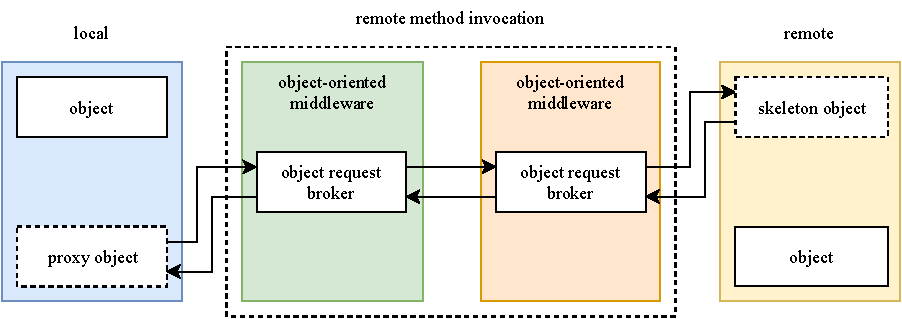
\includegraphics[width=0.8\linewidth]{images/rmi.pdf}
    \caption{A schematic for RMI.}%
    \label{fig:rmi}
\end{figure}

\begin{definition}[Distributed object communication]
    \textbf{Distributed object communication} (DOC) realises
    communication between \textbf{distributed objects}
    (objects spanning multiple address spaces).
\end{definition}

\begin{remark}
    The main idea is to allow objects to access data
    and invoke methods on remote objects.
\end{remark}

\begin{definition}[Remote method invocation]
    \textbf{Remote method invocation} is where a local object
    invokes a method on a remote object.
\end{definition}

\begin{example}[Java RMI]
    Java has an implementation of \emph{object-to-object} communication
    among Java objects to utilise a distributed system.
    RMI allows us to distribute our objects on various machine
    and invoke methods on the objects located on remote
    sites.
    
    An advantage of this is to dynamically create new versions
    of remote objects. 
    This allows us to utilise better suited specialised resources.
\end{example}

When developing a RMI-based app we must design the
interface for the service and then implement the methods specified
in the interface.

On run time, the server will dynamically generate the stub and
register the service by name and location.
The client will look up remote reference on the registry and
use the service in an application.

Host machines has registries that names and looks up remote objects.

Servers can register their objects and clients can find server
objects (by name) and obtain a remote reference from a registry.
Clients can also obtain stubs for a remote object and can also
request a list of remote objects from the registry.

\paragraph{Properties and limitations of DOC}
\begin{enumerate}
    \item 
        DOC follows an object-oriented programming models,
        so allows encapsulation and inheritence.

    \item  
        DOC has the same limitations in terms of connection timeout.

    \item 
        Object request brokers maps object references
        to physical locations; hence, we can meet our location
        transparency requirement.

    \item 
        Services comprising of multiple servers are easier to build
        as all server can be acquired through the object request
        broker.
        Geographical complexity and changes of services are hidden.
\end{enumerate}
